\documentclass[wcp]{jmlr}

\usepackage{enumerate}
\usepackage{bbold}
\usepackage{booktabs}
\usepackage{natbib}
\usepackage[utf8]{inputenc}

 % The following command is just for this sample document:
\newcommand{\cs}[1]{\texttt{\char`\\#1}}


 % change the arguments, as appropriate, in the following:
%\jmlrvolume{1}
%\jmlryear{2014}
%\jmlrworkshop{\textcolor{red}{Neural Connectomics Workshop}}
\jmlrproceedings{}{}

\title{Simple connectome inference from partial correlation statistics in calcium imaging}

\author{Antonio Sutera,
        Arnaud Joly,
        Vincent François-Lavet,
        Aaron Qiu, \\
        Gilles Louppe,
        Damien Ernst,
        Pierre Geurts}

 % Authors with different addresses:
 % \author{\Name{Author Name1} \Email{abc@sample.com}\\
 % \addr Address 1
 % \AND
 % \Name{Author Name2} \Email{xyz@sample.com}\\
 % \addr Address 2
 %}

\editor{Editor's name}
 % \editors{List of editors' names}

\begin{document}

\maketitle

\begin{abstract} In this work, we propose a simple, but yet efficient, method for the problem of connectome inference in
calcium imaging data. The proposed algorithm is made of two steps. First,
processing the raw signals to detect neural peak activities. Second, inferring
the degree of association between neurons from partial correlation statistics.
This paper summarizes the methodology that led us to win the Connectomics
Challenge, proposes a simplified version of our method and finally discusses
our results with respect to other inference methods.\end{abstract}

\begin{keywords}
Connectomics - Network inference - Partial correlation
\end{keywords}


\section{Introduction}\label{sec:intro}

%%%%%%% !!!!!!!! \textcolor{red}{To improve (style):} !!!! %%%%%%%%
The human brain is a complex biological
organ made of 100 billions of neurons, each connected to 7000 other neurons on
average. Unfortunately, direct observations of the connectome, the wiring
diagram of the brain, is not yet technically feasible. Without being perfect,
calcium imaging currently allows the real-time and simultaneous observation of
neuron activities from thousands of neurons, producing individual time series
representing their fluorescence intensity. From these data, the connectome
inference problem consists in retrieving the synaptic connections between
neurons on the basis of the fluorescence time series. In particular, this
problem is often made difficult because of experimental issues, including
masking effects (making some of the neurons not to be observed or confounded
with others), the low sampling rate of the optical device with respect to the
neural activity speed or the slow decay of fluorescence.
%%%%%%%%%%% !!!!!!!!!!!!!! %%%%%%%%%%%%%%%%

Formally, the connectome can be represented as a directed graph $G=(V,E)$,
where $V$ is a set of $p$ nodes, representing neurons, and $E \subseteq
\left\{(i, j) \in V \times V\right\}$ is a set of edges, representing direct
synaptic connections between neurons. Causal interactions are expressed by the
direction of edges: $(i, j) \in E$ indicates that the state of neuron $j$ might
be caused by the activity of neuron $i$. In those terms,  the connectome
inference problem is formally stated as follows:  \textit{Given the sampled
observations $\{ x^t_i \in \mathbb{R} | i \in V, t = 1, \dots, T \}$ of $p$
neurons for $T$ time intervals, the goal is to infer the set $E$ of connections in $G$.}

In this paper, we present a simplified -- yet nearly as good -- version of the
winning method\footnote{Code available at \url{https://github.com/asutera
/kaggle-connectomics}} of the Connectomics
Challenge\footnote{\url{http://connectomics.chalearn.org}}, as a simple and
theoretically grounded approach based on signal processing techniques and
partial correlation statistics. The paper is structured as follows: Section
\ref{sec:filter} describes the signal processing methods applied on fluorescent
calcium time series; Section \ref{sec:inference} then presents the proposed
approach and its theoretical properties; Section \ref{sec:results} provides an
empirical analysis and comparison with other network inference methods, while
Section \ref{sec:conclusion} finally discusses our work and provides further
research directions. Additionally, Appendix \ref{app:optimized} further
describes, in all details, our actual winning method, giving slightly better
results than the method presented in the paper, at the price of parameter
tuning.


\section{Signal processing} \label{sec:filter}

Under the simplifying assumption that neurons are on-off units, characterized
by short periods of intense activities, or peaks, and longer periods of
inactivity, the first part of our algorithm consists in cleaning the raw
fluorescence data. More specifically, time series are processed using standard
signal processing filters in order to remove noise due to light scattering
effects, account for fluorescence  low decay and reduce the importance of
global high activity in the network. The overall process is illustrated in
Figure~\ref{fig:filtered-signal}.

\begin{figure}
\centering
\subfigure[Raw signal]{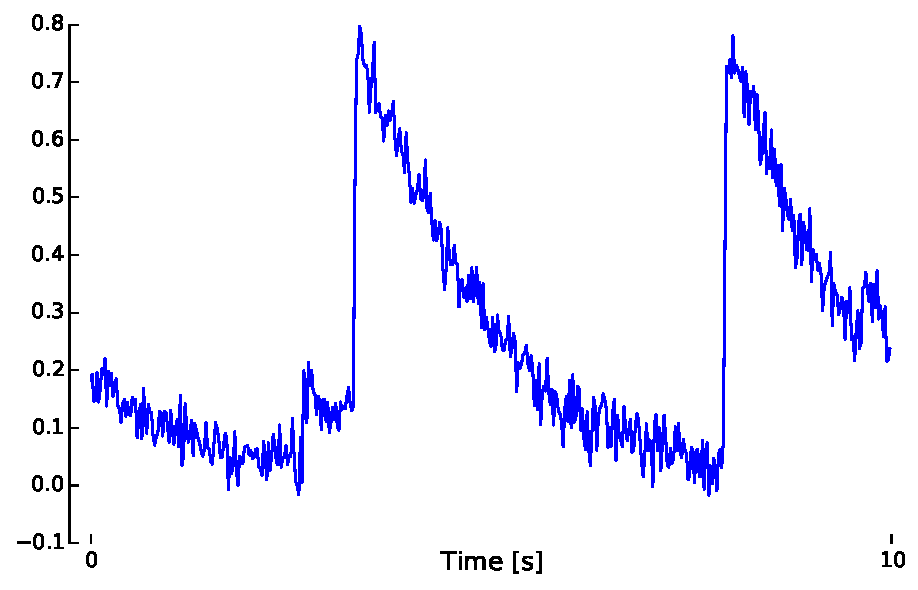
\includegraphics[width=0.3\textwidth]{images/original_curve.pdf} \label{fig:original_curve}}
\subfigure[Low-pass filter $f_1$]{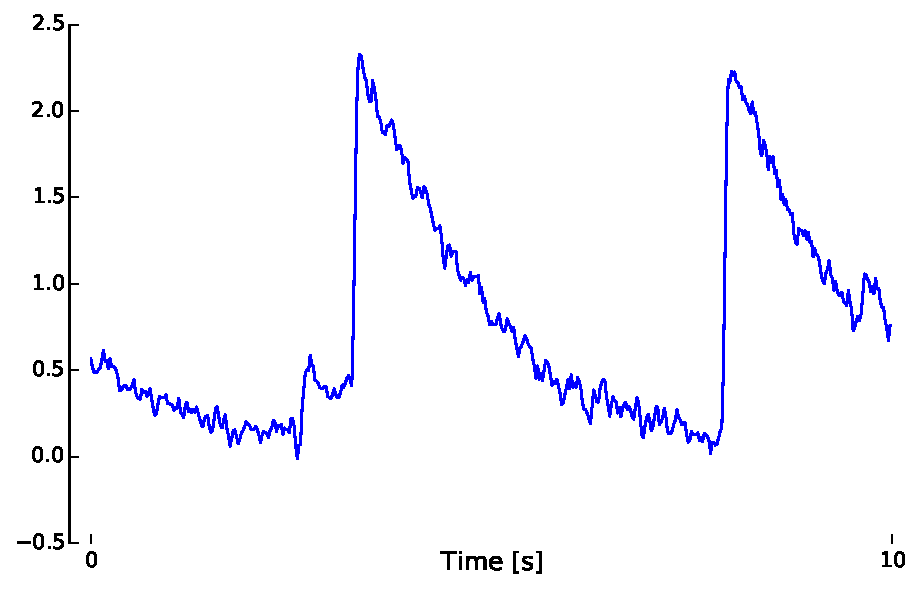
\includegraphics[width=0.3\textwidth]{images/filter_curve.pdf} \label{fig:lp_curve}}
\subfigure[High-pass filter $g$]{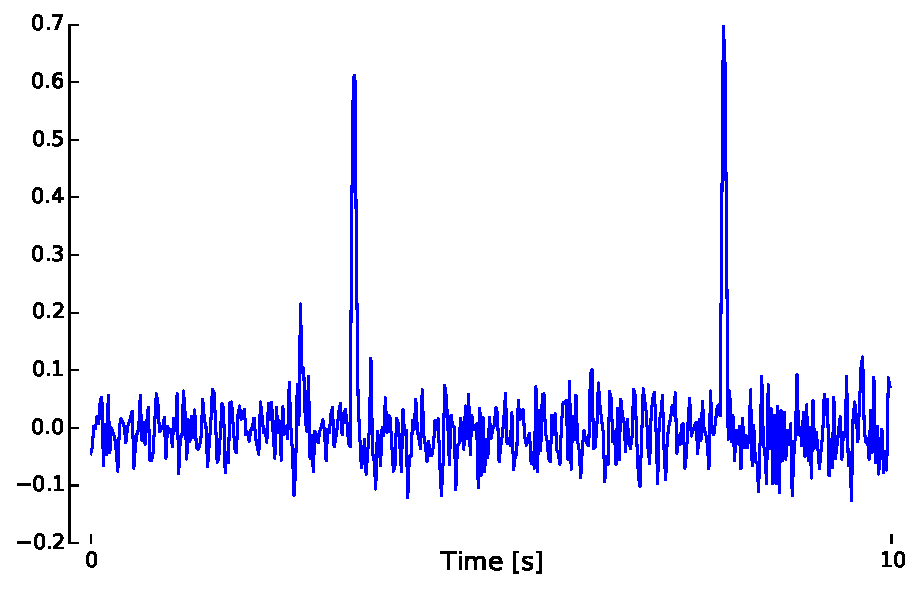
\includegraphics[width=0.3\textwidth]{images/diff_curve.pdf} \label{fig:hp_curve}}\\
\subfigure[Hard-threshold filter $h$]{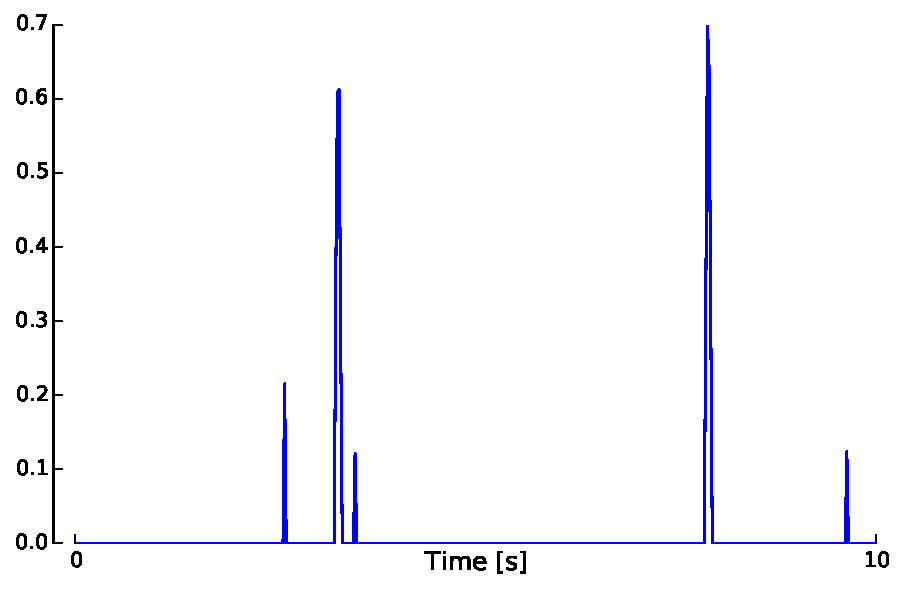
\includegraphics[width=0.3\textwidth]{images/threshold_curve.pdf} \label{fig:threshold_curve}}
\subfigure[Global regularization $w$]{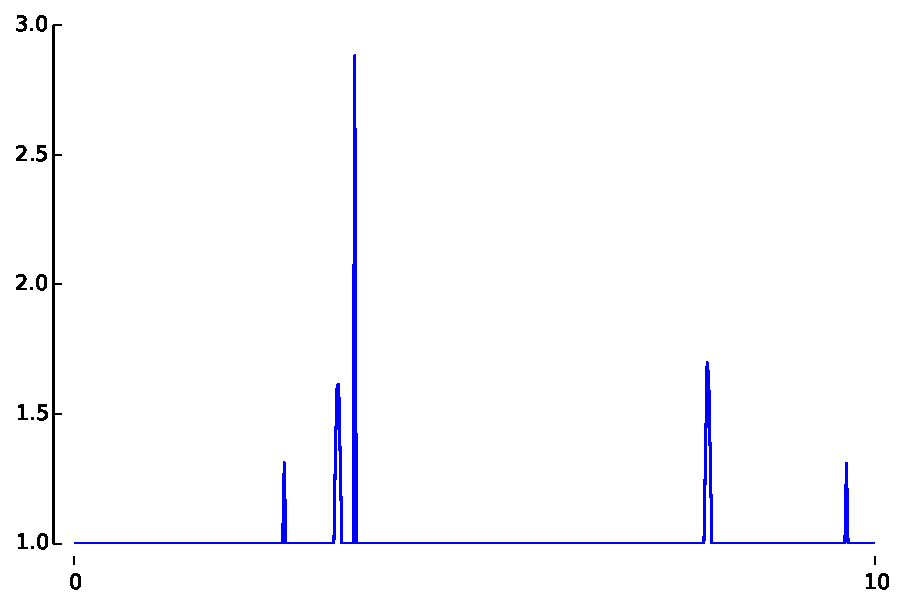
\includegraphics[width=0.3\textwidth]{images/weights_curve.pdf} \label{fig:weight_curve}}
\caption{Signal processing process for extracting peaks from the raw fluorescence data.
         \textcolor{red}{AJ: The bottom axe is hidden on some figures.}}
\label{fig:filtered-signal}
\end{figure}

As Figure~\ref{fig:original_curve} shows, the raw
fluorescence signal is very noisy due to light scattering artifacts that
ordinarily affect the quality of the recording~\citep{lichtman2011big}.
Accordingly, the first step of our pipeline is to smoothen the signal, using
one of the following low-pass filters for filtering out high frequency noise:
\begin{align}
% symmetrical median filter
f_1(x^t_i) &= x^{t-1}_i + x^t_i + x^{t+1}_i \label{eq:symetric-median}, \\
% asymmetrical weighted median
f_2(x^t_i) &= 0.4 x^{t-3}_i + 0.6 x^{t-2}_i + 0.8 x^{t-1}_i + x_i^t.
\label{eq:weighted-asymetric-median}
\end{align}
For the sake of illustration, the effect of the filter $f_1$ on the signal
is shown in Figure \ref{fig:lp_curve}.

Furthermore, it can be observed that neurons communicate through short spikes, characterized by a high
frequency, while low frequencies of the signal mainly correspond to the slow
decay of fluorescence. To have a signal that only has high magnitude around instances where the spikes occur, the second step of our pipeline transforms the time series into its backward
difference
\begin{align}
g(x^{t}_{i}) &= x^{t}_i - x^{t-1}_i \label{eq:high-pass-filter},
\end{align}
as shown in Figure \ref{fig:hp_curve}.

To filter out small variations in the signal obtained after applying the
function $g$ as well as to eliminate negative values, we use the following
hard-threshold filter
\begin{align}
h(x^{t}_i) &= x^{t}_i \mathbb{1}(x^{t}_i \geq \tau) \text{ with } \tau > 0,
\end{align}
yielding Figure \ref{fig:threshold_curve}.
As we can see, the processed signal only contains clean spikes.

The objective of the last step of our filtering procedure is to decrease the
importance of spikes that occur when there is a high global activity in the
network with respect to  spikes that occur during normal activity. Indeed, we
have conjectured that when a large part of the network is firing, the rate at
which observations are made is not high enough for being able to detect
interactions and, that it would therefore be preferrable to lower their
importance by changing appropriatly their magnitude. Additionnally, it is
well-known that neurons may also spike because of a global high activity
\citep{stetter2012model}. In such  context, detecting pairwise neuron
interactions from the firing activity is meaningless. As such,
the signal output by $h$ is finally applied to the following function
\begin{align}
 w(x^{t}_i) &= (x^{t}_i + 1 )^{1 + \frac{1}{\sum_{j} x^{t}_j}},
\end{align}
which effect is to magnify the importance of spikes that occur in case of low global activity (measured by $\sum_{j} x^{t}_j$), as observed for instance around $t=4\text{s}$ in the figure.
Note that the particular case where there is no activity, i.e., $\sum_{j} x^{t}_j = 0$, is solved by setting $w(x^{t}_i) = 1$. 


To summarize, the full signal processing pipeline of our simplified (resp.
tuned) approach is defined by the composed function $w \circ h \circ g \circ
f_1$ (resp. $f_2$). When applied to the raw signal of Figure
\ref{fig:original_curve}, it outputs the signal shown in Figure
\ref{fig:weight_curve}.


\section{Connectome inference from partial correlation statistics}
\label{sec:inference}

% No time assumption

Our procedure to infer connections between neurons first assumes that
the (filtered) fluorescence concentrations of all $p$ neurons at each
time point can be modeled as a set of random variables $X = \{X_1,
\dots, X_p\}$ that are idependently drawn from the same time invariant
joint probability distribution $P_X$. %% Or, say otherwise, we assume
%% that there exists a probability distribution $P_X$ such that the
%% fluorescence concentrations at a particular time $t$ can be seen as an
%% independent realization of $P_X$.
As a consequence, our inference method does not exploit the time
ordering of the observations (although time ordering is exploited by
the filters).

% partial correlation: definition + motivation

Given this assumption, we then propose to use as a measure of the
strength of the connection between two neurons $i$ and $j$, the
partial correlation coefficient $p_{i,j}$ between their corresponding
random variables $X_i$ and $X_j$, defined by \cite{}:
\begin{equation}
p_{i,j} =
-\frac{\Sigma^{-1}_{ij}}{\sqrt{\Sigma^{-1}_{ii} \Sigma^{-1}_{jj}}}, \label{eq:inverse}
\end{equation}
where $\Sigma^{-1}$, known as the precision or concentration matrix, is the inverse of the covariance matrix $\Sigma$ of $X$.%%  Partial
%% correlation can be interpreted in several ways. The partial
%% correlation coefficient $p_{i,j}$ can be shown to measure the
%% correlation between $X_i$ and $X_j$ when they are corrected for the
%% (linear) effect of all other variables in $X$ \cite{}.
Assuming that the distribution $P_X$ is a multivariate Gaussian
distribution ${\cal N}(\mu,\Sigma)$, it can be shown that $p_{i,j}$ is
zero if and only if $X_i$ and $X_j$ are independent given all other
variables in $X$, ie. $X_i \perp X_j|X^{-i,j}$ where $X^{-i,j}= X
\setminus\{X_i,X_j\}$. Partial correlation thus measures conditional
dependencies between variables. As an association measures between
neurons, it should thus naturally only detect direct associations
between neurons and filter out spurious indirect effects. The interest
of partial correlation as an association measure has already been
shown for the inference of gene regulatory networks \cite{xxx}.
%% Given a set of multivariate Gaussian
%% random variables $X$, the (undirected) graph that connects all pairs
%% of variables $X_i$ and $X_j$ such that $p_{i,j}\neq 0$ is called a
%% Gaussian graphical models (GGMs). Because it measures conditional
%% dependencies, partial correlation should naturally only detect direct
%% associations between neurons. The superiority of partial correlation
%% over standard correlation as an association measure have already been
%% shown in the context of the inference of gene regulatory networks from
%% gene expression data \cite{}. We will compare both measures in Section
%% \ref{sec:results}.
Note that the partial correlation statistic is symmetric
(i.e. $p_{i,j}=p_{j,i}$). Therefore, our approach cannot identify the
direction of the interactions between neurons. We will see in
Section~\ref{sec:results} why this only affects slightly its
performances, with respect to the metric used in the Connectomics
challenge.

Practically, the computation of coefficient $p_{i,j}$ using Equation
\ref{eq:inverse} requires the estimation of the covariance matrix $\Sigma$
and then computing its inverse. Given that we have typically more
samples than neurons, the covariance matrix can be inverted in a
straightforward way. We nevertheless obtained some improvement by
replacing the exact inverse with an approximation using only the $M$
first principal components of $\Sigma$~\citep{bishop2006pattern} (with
$M$ set to $0.8 p$ in our experiments).

Finally, let us remark that performance of our simple method shows to
be quite sensitive to the values of parameters (e.g., $f_1$ or $f_2$
or the value of the threshold $\tau$) in the combined function of the
filtering and infering processes. One approach, that we will refered
to as \textit{Averaged Partial correlation} statistics, for improving
its robustness is to average correlation statistics over various
values of the parameters, thereby reducing the variance of its
predictions. Further details about parameter selection are provided in
Appendix~\ref{app:optimized}.

% Note on directionality


%% Our  connection inference  procedure  relies  on several  assumptions. First,
%% we will assume that  the fluorescence concentrations of all $p$ neurons can be
%% modeled as a set of random variables $X = \{X_1, \dots, X_p\}$  that are drawn
%% from a time invariant joint  probability distribution $P_X$. Or, say otherwise,
%% we assume that there exists a probability distribution $P_X$ such that the
%% fluorescence concentrations at a particular time $t$ can be seen as an
%% independent realization of $P_X$.

%% To assess the presence of a connection between two neurons, we will
%% use partial correlation statistics, which has been used extensively
%% for the inference of gene regulatory networks \cite{}.


%% To a joint probability distribution $P_X$ corresponds a
%% graph where (i) each node is a random variable and (ii) two nodes are
%% only connected if they correspond to two dependent variables. We assume that two neurons are
%% connected if  and only if,  there exists  in this  graph an edge
%% that connects  directly the  two random  variables to  which they correspond.
%% In this context, it is equivalent to writing that two neurons $i$ and $j$ are  not  directly
%% connected  if and only if  $X_i$  and $X_j$  are  conditionally independent
%% with  respect to all  other variables. We remind  that two random  variables
%% $X_i$  and  $X_j$  are  said  to  be  conditionally independent to a (possibly
%% empty)  set of controlling random variables $Z$, denoted $X_i \perp X_j | Z$,
%% if the joint conditional probability distribution   $P_{X_i,  X_j   |   Z}$
%% factorizes  into   $P_{X_i|Z} P_{X_j|Z}$.  In particular,  when  $X_i$ and
%% $X_j$ are  conditionally independent  with respect  to all  the other
%% variables, denoted  $X_i \perp  X_j  | X^{-i,j}$,  then  the  observation  of
%% $X_i$  given  the knowledge  of  $X^{-i,j}$ provides  no information  about
%% $X_j$,  and vice-versa.

%% In the  particular case where $P_X$ is  a joint  Gaussian distribution
%% $\mathcal{N}(\mu; \Sigma)$ of mean  vector $\mu$ and covariance matrix
%% $\Sigma$, $X_i$  and $X_j$ are conditionally  independent with respect to the
%% other variables $X^{-i,j}$ if their \textit{partial correlation} statistic is
%% null~\citep{baba2004partial}, i.e., if
%% \begin{equation}
%% \rho_{X_i, X_j | X^{-i,j}} = -\frac{\Sigma^{-1}_{ij}}{\sqrt{\Sigma^{-1}_{ii} \Sigma^{-1}_{jj}}} = 0, \label{eq:inverse}
%% \end{equation}
%% where $\Sigma^{-1}$ is known as the precision or concentration matrix.
%% Conversely, $X_i$ and $X_j$ are conditionally dependent if $\rho_{X_i, X_j |
%% X^{-i,j}} \neq 0$, where $\rho_{X_i, X_j | X^{-i,j}} \in [-1;1]$. Note that the
%% larger the value of this term, the stronger the dependence between variables
%% $X_i$ and $X_j$.

%% Our approach implicitly makes the additional assumption  that $P_X$ is  a
%% joint Gaussian distribution since it  outputs as degree of association
%% between two neurons $i$ and $j$ an estimate of $\rho_{X_i, X_j | X^{-i,j}}$.
%% Note also that the partial correlation
%% statistic is symmetric  (i.e., $\rho_{X_i, X_j | X^{-i,j}} = \rho_{X_j, X_i |
%% X^{-j,i}}$). Therefore, our approach cannot identify the direction of the interaction. We will see in Section~\ref{sec:results} why this only affects slightly its performances, with respect to the metric used in the Connectomics challenge.

%% We now detail our procedure for estimating partial correlation
%% statistics ($\rho_{X_i, X_j | X^{-i,j}}$) from the data. It first
%% estimates the covariance matrix from the data. Afterwards, it computes
%% the exact inverse of this matrix, from which it infers the value of
%% $\rho_{X_i, X_j | X^{-i,j}}$ using equation (\ref{eq:inverse}). Note
%% that we have also experimented procedures where the exact inverse was
%% replaced by an approximation of it using only the $M$ principal
%% components of $\Sigma$~\citep{bishop2006pattern} whose associated
%% eigen values were significantly higher than zero. Such an
%% approximation is equivalent to assume that the firing activity of all
%% neurons can be explained by only a subset of them whose size is equal
%% to $M$. We observed that those procedures were often leading to better
%% results. Note that we found out by running expriments that the number
%% $M$ of principal components is around $0.8p$ (see discussion in
%% Appendix~\ref{app:REF} \textcolor{red}{REF}).

%% % Computationally, they can be estimated
%% % % efficiently in $O(M^3)$ (instead of $O(p^3)$)
%% % from the $M$ first principal
%% % components extracted through PCA~\citep{bishop2006pattern} on the processed
%% % data. While speeding up computation, it allows to further
%% % filter the the data by removing the contribution of components that are respectively
%% % due to redundancy or noise, i.e., with an eigen value respectively is equal to zero or close to zero.

\section{Experiments} \label{sec:results}

%% \textcolor{red}{to incorporate:
%% To highlight the benefits of measuring the partial dependence conditional to
%% all other variables, we compare in Section~\ref{sec:results} with the
%% \textit{Pearson correlation} statistics, which measure instead the linear
%% dependence between variables, independently of the others. Accordingly, $X_i$
%% and $X_j$ are independent, without any conditioning, if their Pearson correlation statistic is zero, that
%% is if
%% \begin{equation}
%% \rho_{X_i,X_j} = \frac{\Sigma_{ij}}{\sqrt{\Sigma_{ii} \Sigma_{jj}}} = 0.
%% \end{equation}}

\paragraph{Data and evaluation metrics.}

We report here experiments on the \textit{normal}-1,2,3, and 4
datasets provided by the organizers of the Connectomics
challenge. Each of these datasets is obtained from the simulation
\citep{stetter2012model} of different neural networks of 1000 neurons
and about 15000 edges each (ie., a network density of about
1.5\%). Each neuron is described by a calcium fluorescence time series
of length $T=179500$. All inference methods compared here provide a
ranking of all pairs of neurons according to some association
score. To assess the quality of this ranking, we compute both ROC and
precision-recall curves against the ground truth network, which are
summarized using the area under the curve, denoted respectively AUROC
and AUPRC. Only the AUROC score was used to rank the challenge
participants but the precision-recall curve has been shown to be a
more sensible metric for network inference, especially when network
density is small (see e.g. \cite{schrynemackers2013protocols}).
Since neurons are not self-connected in the ground truth networks
(ie., $(i, i) \not \in E, \forall i \in V$), we have manually set the
score of such edges to the minimal possible association score before
computing ROC and PR curves.

\paragraph{Evaluation of the method}

The top of Table \ref{tab:comparison} reports AUROC and AUPRC for all four networks
using in each case partial correlation with different filtering
functions. Except for the last two rows that uses PCA, the exact
inverse of the covariance matrix was used in each case. These results
clearly show the importance of the filters. AUROC increases in average from
0.77 to 0.93. PCA does not really affect AUROC scores but it improves
significantly AUPRC scores. Taking the average over various parameter
setting gives an improvement of 10\% in both AUROC and AUPRC. The last
row shows the final performance of the method specifically tuned for
the challenge (see the Appendix for all details). Although this tuning
was decisive to obtain the best performance at the challenge, it does
not significantly improve neither AUROC nor AUPRC. Note that tuning
was mainly done on the \textit{normal-1} and \textit{normal-4}
datasets, which explains why these two networks are slightly better
retrieved than the others.

\begin{table}[t]
\caption{Evaluation of different methods on the four \textit{normal} datasets\label{tab:comparison}}
\centering
\small
\begin{tabular}{@{}l *{8}{c}@{}}
\hline
  & \multicolumn{4}{c}{AUROC} & \multicolumn{4}{c}{AUPRC} \\
\hline
Methods $\backslash$ normal- & 1 & 2 & 3 & 4 & 1 & 2 & 3 & 4 \\
No  filtering       					& 0.777 & 0.767 & 0.772 & 0.774 & 0.070 & 0.064 & 0.068 & 0.072\\
$ h \circ g \circ f_1$                  & 0.923 & 0.925 & 0.923 & 0.922 & 0.311 & 0.315 & 0.313 & 0.304\\
$ w \circ h \circ g \circ f_1$          & 0.931 & 0.929 & 0.928 & 0.926 & 0.326 & 0.323 & 0.319 & 0.303\\
+ PCA         							& 0.932 & 0.930 & 0.928 & 0.926 & 0.355 & 0.353 & 0.350 & 0.333\\
Averaging           					& 0.938 & 0.936 & 0.936 & 0.932 & 0.391 & 0.389 & 0.385 & 0.374\\
Full method           					& 0.943 & 0.942 & 0.942 & 0.939 & 0.403 & 0.404 & 0.398 & 0.388\\
\hline
Correlation & 0.886 & 0.884 & 0.891 &  0.877 & 0.153 & 0.145 & 0.170 & 0.132\\
GTE & 0.890 & 0.893 & 0.894 & 0.873 & 0.171 & 0.174 & 0.197 & 0.142\\
GENIE3 &\\
\end{tabular}
\caption{TODO \textcolor{red}{version simple!!}}
\label{tab:tab3}
\end{table}




\paragraph{Comparison with other methods}

In the bottom of Table \ref{tab:comparison}, we provide as a comparison the
performance of three other methods: standard (Pearson) correlation (PC),
generalized transfer entropy (GTE), and GENIE3. ROC and PR curves on the
\textit{normal-2} network are shown for all methods in Figure
\ref{fig:}. Pearson correlation measures the unconditional linear
(in)dependence between variables and it should thus not be able to filter out
indirect interactions between neurons. GTE \citep{stetter2012model} was
proposed as a baseline for the challenge. This method builds on Transfer
Entropy to measure the association between two neurons. Unlike our approach, it
can predict the direction of the edges. GENIE3 \citep{huynhthu2010inferring} is
a gene regulatory network inference method that was the best performer of the
DREAM5 challenge \cite{dream5paper}. When transposed to neural networks, this
method uses as a confidence score for the edge going from neuron $i$ to neuron
$j$ the importance score of variable $X_i$ in a Random Forests model trying to
predict $X_j$ from all variables in $X\setminus X_j$. To reduce computing times
of this method, we had to reduce each tree in the Random Forests model to a
maximum depth of 3. This constraint potentially severly affects the performance
of this method with respect to the use of fully grown trees. We nevertheless
provide these results for comparison purpose. PC and GENIE3 were both applied
on the same pre-filtered time series ($g \circ f_1$). For GENIE3, we
built 10000 trees per neuron and we used default settings for all other
parameters (except for the maximal tree depth). For GTE, we reproduced the
exact same setting (conditioning level and pre-processing) that was used for
the challenge.

%% To assess our method, we focus on the \textit{normal-2} dataset
%% provided by the organizers of the Connectomics challenge. Experiments
%% on \textit{normal-1, normal-3, normal-4} show similar trends to
%% \textit{normal-2} and are presented in the Appendix \textcolor{red}{REF}.
%% Those datasets have $p=1000$ time series of length $T=179500$ of image
%% calcium from simulated neuronal networks \citep{stetter2012model}. Each of these
%% networks contains approximately 15000 edges.

%% % Metrics : ROC AUC and AUPRC
%% In supervised learning terms, the network inference task can be viewed as a
%% binary classification task where one has to correctly classify the presence or
%% the absence of edges of the graph. We assess the accuracy of the network
%% inference method using the area under the ROC curve (AUROC) and the area under
%% the precision-recall curve (AUPRC) \citep{schrynemackers2013protocols}.


%% The proposed approach is compared to Pearson correlation statistics
%% (as described in Section~\ref{sec:inference}), generalized transfer
%% entropy (GTE) and the GENIE3 algorithm.
%% \begin{itemize}
%% \item \textbf{GTE} \citep{stetter2012model}, the baseline of the challenge,
%% measures for all pairs of neurons $i$ and $j$ the reduction of uncertainty in
%% predicting future values of $i$ given the observation of the time series of the
%% neuron $j$ conditionally to the observation of past time series of neuron $i$,
%% whenever the average fluorescence is over a conditioning level. Pre-processing
%% and conditioning level were set to reproduce baseline of the challenge.

%% \item \textbf{GENIE3} \citep{huynhthu2010inferring} translates the inference
%% of the network of $p$ neurons into $p$ supervised learning tasks. For each
%% task, the fluorescence of a neuron is predicted from the fluorescence of all
%% other neurons using a tree based ensemble such as random forest
%% \citep{breiman2001random}. The tree ensemble associates a variable importance
%% score \citep{louppe2013understanding} to each neuron used in the predictions,
%% which is used as a degree of associate. The following parameters are used
%% $10000$ trees, $\log_2{p}$ variables are randomly selected to split tree nodes
%% and the maximal tree depth is constrained to 1, 2 or 3. \textcolor{red}{AJ Which
%% depth is represented on the graph?}
%% \end{itemize}

%% \subsection*{Partial correlation improves over state-of-the-art methods}

Partial correlation and average partial correlation clearly outperforms all
other methods. The improvement is more important in terms of AUPRC than in
terms of AUROC. As expected, Pearson correlation performs very poorly in terms
of AUPRC. GTE and GENIE3 works much better but these two methods are
nevertheless clearly below partial correlation. Among these two methods, GTE is
slightly better in terms of AUROC, while GENIE3 is significantly better in
terms of AUPRC. Given that we had to limit this latter method for computational
reasons, these results are very promising and a comparison with the full GENIE3
approach is certainly part of our future works.

%% bu by about a factor
%% of 2 in AUPRC reaching $0.347$ and an increased of $0.03$ in
%% AUROC. Averaging Partial correlation matrix over a wide of parameters
%% further improves AUPRC to $0.389$ and improve AUROC by $0.009$.  Two
%% reasons might explain such differences: (i) only the partial
%% correlation-based methods and GENI3 at lesser extent distinguish
%% direct links from indirect one, (ii) simulated networks from the
%% \citep{stetter2012model} generator or neural networks in general could
%% be reduced to a linear model after pre-processing. Those results
%% generalizes over the other datasets see Appendix \textcolor{red}{REF}.

\begin{figure}[t]
\centering
\subfigure[ROC curves]{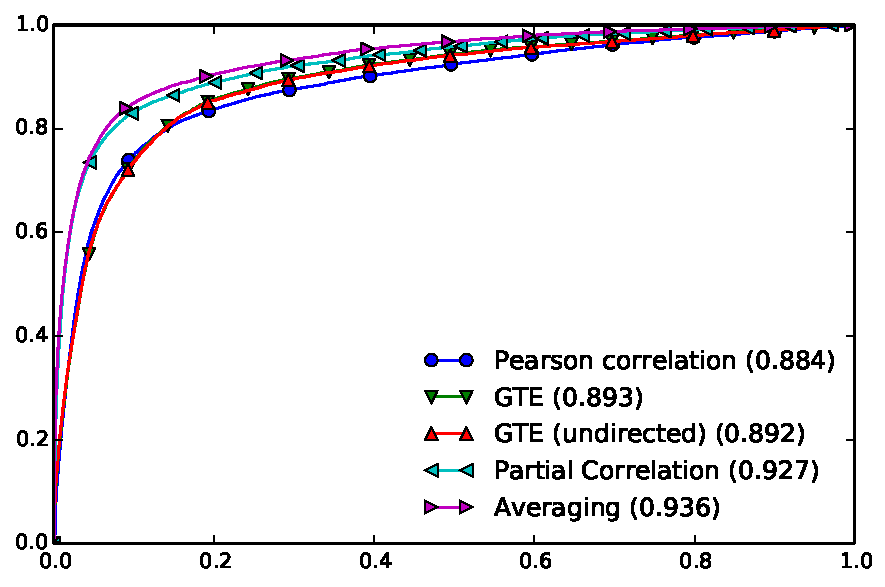
\includegraphics[width=0.45\textwidth]{images/curve_roc} \label{fig:roc_curve}}
\subfigure[Precision-recall curves]{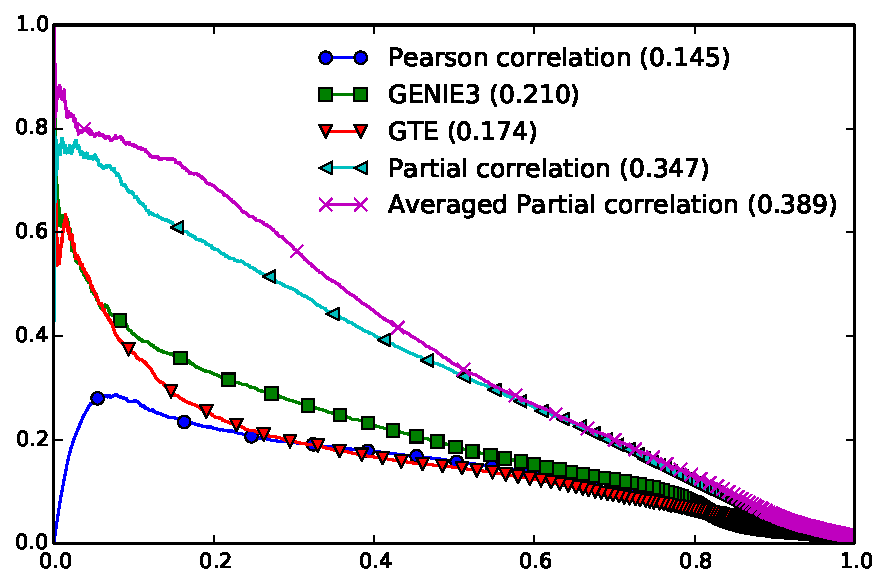
\includegraphics[width=0.45\textwidth]{images/curve_pr} \label{fig:pr_curve}}
\caption{ROC (left) and PR (right) curves on \text{normal-2} with different methods. Area under the curves are reported in the legend for each method.}

%% The weighted average of partial correlation matrix, winning approach
         %% of the challenge, yields better than AUROC and AUPRC than all
         %% other state-of-the-art methods. (parameters: $\tau=0.11$ except for
         %% averaged partial correlation method, partial correlation used
         %% filter $f_1$). Area under the curves are given between $()$
         %% for the corresponding methods.
%}
\label{fig:curves}
\end{figure}

%% \textcolor{red}{Only one GENI3, thus it can't be observed.}
%% As observed on Figure \ref{fig:curves}, the GENIE3 performance increases with
%% deeper trees while being still computationally feasible. The reason is twofold.
%% First, the deeper the tree, the larger is the conditioning. \textcolor{red}{AJ:
%% conditioning?} As it was observed in the comparison between correlation and
%% partial correlation, it screens indirect links in the inferred network.
%% \textcolor{red}{AJ: I don't understand the link with GENIE3} Second, the number
%% of small trees need to be much higher than deep trees in order to observe - and
%% evaluate - all pairs.  However, as suggested by \cite{louppe2014understanding},
%% limiting the maximal depth of trees may help to improve the variable importance
%% computing, i.e. inferring the degree of association. \textcolor{red}{AJ: there
%% is no explanation of why it would be better apart for computational reason.}
%% Therefore a trade-off  of the maximal depth may give the best of both worlds.
%% \textcolor{red}{AJ:  Which tradeoff? Which worlds?}


\subsection*{ROC versus PR curves}

%% The best method only infers the \textbf{undirected} network by giving the same
%% degree of association to both edges $(i,j)$ and $(j,i)$. This is quite
%% surprising considering the problem statement. Trying to direct links could be
%% more penalizing than rewarding. For example, symmetrizing the degree of
%% association matrix does not necessarily degrade AUPRC and AUROC.


%% If the inferred network corresponds to the undirected network, it would
%% already yield high AUROC score for instance $\approx 0.996$ on
%% \textit{normal-1}. Infering edge directivity is likely to be counter-
%% productive or yield small gain. By contrast, the same experiment with AUPRC
%% would yield a score of $\approx 0.789$ on \textit{normal-1}. Thus inferring
%% correctly directivity would be more rewarding in AUPRC term.

%% % Interestingly, methods that takes into account directivity, namely GTE and
%% % GENIE3, improve their AUROC and AUPRC by giving the same way to directed edges.
%% % (in particular see GTE and GTE(undirected) in Figure \ref{fig:pr_curve}
%% % \textcolor{red}{AJ: Figure \ref{fig:curves}  contradicts this message,
%% % especially pr-curve. AS:And now?} and Table \ref{tab:tab1} in Appendix \textcolor{red}{REF}).
%% % Trying to detect the link direction is more penalizing than rewarding.

%% The area under the ROC curve is not a consistent metric with respect to the
%% problem statement. A clear hierarchy is also difficult to derive from ROC
%% curves as shown on Figure \ref{fig:roc_curve}. We advice to avoid the AUROC for
%% the assessment of network inference method. An alternative would be to assess
%% network inference using the area under the precision-recall curve (AUPRC).
%% Those conclusions are in line with \cite{schrynemackers2013protocols}.


\section{Conclusions} \label{sec:conclusion}


% Possible extensions
% partial autocorrelation function (sometimes "partial correlation function")
% conditional independence test
% Speak about the complexity and parallelization of the methods

In this paper, we present the best performing method of the Connectomics challenge. Our
approach is simple and theoretically sounded and made of two main stages: the
signal is first preprocessed with several filters and then we derive the degree
of association matrix by computing the partial correlation statistics matrix.
We also evaluate the method in a more detailed way and perform a comparison
with other inference methods. We finally discuss the relevance of the metric
used in the challenge and we point out that it was not necessary to discover
causal relationships to maximize the ROC AUC. Thus, it may be  promising to
focus on that particular topic in future works.

% In the discussion, we give hints about limiting the depth of trees in the
% GENIE3 method to infer the network. It should be interesting to see if there
% is a optimum value for the maximal depth. And of course, it may also rewarding
% to increase considerably the number of trees to get more stable predictions.

% In previous study \citep{shipley2002cause}, it has been suggested to
% consider correlation coefficients of all possible orders,
% i.e. conditioned on every subsets of the set of $p-2$ other variables. This
% would take into account multiple indirect paths between a given pair of
% variables. Instead of considering only the highest order, it may be useful to
% study with accuracy the inferred network at all orders. In this case, it may not
% be very relevant but interesting in case of dynamical networks.

% As we mentioned, in order to maximize the ROC AUC, it was not necessary to
% discover causal relationships. It may be, in future works, promising to focus
% on that particular topic.


\section*{Acknowledgments}
A Joly and G Louppe are research fellows of the FNRS, Belgium.  A Sutera is
recipient of a FRIA fellowship of FRS-FNRS, Belgium. This work is supported by
PASCAL2 and the IUAP DYSCO, initiated by the Belgian State, Science Policy
Office.



\newpage
\clearpage

% We allow the bibliography to be added on top of the 6 pages.
% Supplementary material may be added in the form or a URL pointed to from
% the paper.

\bibliography{references}

\newpage
\clearpage

\appendix


\section{An optimized version of the algorithm to win the challenge}
\label{app:optimized}

Sections~\ref{sec:filter}~to~\ref{sec:results} describe a simplified version
of the actual winning method. However, one could be interesting in the full
description. This appendix will therefore follow the progress of the main
paper highlighting optimizations.

Let us remark that parameter value choices were made to maximize ROC AUC score
on \textit{normal-1} and, to a lesser extent, \textit{normal-4}.

\subsection*{Signal processing}

As we introduce a composed function in section~\ref{sec:filter}, let us describe a new composed function with optimized filters to improve the quality of the inference process.


Besides filters
$f_1$ and $f_2$ respectively defined by equations \ref{eq:symetric-median} and \ref{eq:weighted-asymetric-median}, we also consider two other low-pass
filters:

\begin{align}
f_3(x^t_i) &= x^{t-1}_i + x^{t}_i + x^{t+1}_i + x^{t+2}_i \label{eq:asymetric-median-forward}, \\
f_4(x^t_i) &= x^{t+3}_i + x^{t+2}_i + x^{t+1}_i + x_i^t.
\label{eq:asymetric-median}
\end{align}

Theses filters, even if individually they lead to less good performances of the inference algorithm than filters $f_1$ and
$f_2$, the averaging approach over these four low-pass
filters gets better.

As a computation trick, it appears that using a parametrized hard-threshold filter slighlty improves performances. Introducing the parameter $c$ in function $h$ yields to an optimized filter denoted as $h^*$ \begin{align}
h^*(x^t_i) = (x_i^t)^c \text{ } \mathbb{1}(x_i^t \ge \tau) \text{ with } \tau > 0,
\end{align}
where $c$ is set to $0.9$ after experiments.

The magnification can also be optimized by adjusting the effect differently with respect to the global activity. In that sense, we introduce the following function \begin{align}
 w^*(x^{t}_i) &= {(x^{t}_i + 1 )^{\left (1 + \frac{1}{\sum_{j} x^{t}_j}\right )}}^{m}
\end{align}
where $m$ is a piecewise linear function depending on the low-pass filter and on the range of the global activity. We refer to our implementation\footnote{available on \url{https://github.com/asutera/kaggle-connectomics}.} for the values of the parameters and especially the parameter $m$.

\subsection*{Averaging the connectome inference from partial correlation statistics}

In our experiments, we observed that the inference process is quite sensitive
about the choice of the parameter value $\tau$ and the low-pass filter.
Therefore, in order to reduce the variance of the results and thus the
robustness of our approach, we perform an average over a range of parameter
value $\tau$ from $0.100$ to $0.209$. We also perform a weighted average over
the four low-pass filters with weights  $weight_{f_1} = 1$, $weight_{f_2} =
0.9$, $weight_{f_3} = 0.7$ and $weight_{f_4} = 0.01$, tuned to maximize the
ROC AUC on \textit{normal-1}. The weights were adjusted to take into account
that some filters outperform other but there is information hold in every
filter.



\subsection*{Connectome inference from pairwise interaction statistics}

Since partial correlation statistics is a symmetric measure and the connectome
is a directed graph, it should be rewarding to detect the edge orientation. In
this section, we will present a heuristic trying to retrieve directivity.
However, considering the argument in Section \ref{sec:results}, the additional
gain margin of this approach compared to the undirected method is extremely
limited.

The heuristic is based on the following observation. The rise of fluorescence
of a neuron indicates its activation. If another neuron is activated after a
slight delay, this could have been caused by the activation of the first
neuron and therefore highlight a (direct) directed relationship between the
two neurons. With that in mind, the heuristic principle is to count the number
of such events occurred between neurons $i$ and $j$ for consecutive time
steps. It can be done by counting the number of times that a transition from
neuron $i$ to neuron $j$ for two consecutive time steps, or mathematically we
compute for each pair $(i,j)$

\begin{align}
s_{ij} = \sum_{t=1}^{T - 1} \mathbb{1}((x_j^{t+1} - x_i^t) \in \left[\phi_1, \phi_2\right])
\end{align}
where $\phi_1$ and $\phi_2$ are parameters of the heuristic.

Two issues may be spotted. First, this heuristic is not able to distinguish a
directed relationships if both neurons are activated in the same time step and
may wrongly characterize indirect relationships because of the time
resolution. Second, it may be necessary to take into account $s_{ji}$ to
estimate the quality of the pairwise coefficient $s_{i,j}$. Indeed, if both
coefficients are similar ($s_{ij} \sim s_{ji}$) the directivity can not be
inferred since the order of fluorescent rising is not well defined. On the
contrary, different coefficients $s_{ij}$ and $s_{ji}$ mean that an order of
fluorescent rising is well established and observable. There we choose to
compute a differential pairwise coefficient $z_{ij}$ defined by the following
equation


\begin{align}
z_{ij} = \sum_{t=1}^{T - 1}
    \mathbb{1}((x_j^{t+1} - x_i^t) \in \left[\phi_1, \phi_2 \right]) -
    \mathbb{1}((x_i^{t+1} - x_j^t) \in \left[\phi_1, \phi_2 \right]),
\end{align}
where $T$ is the number of time steps, $\phi_1$ and $\phi_2$ are parameters.

At the light of the poor results of this heuristic taken on its own summarized
on Table \ref{tab:} as \textit{directivity}, we use it to make asymmetric the
degree of association matrix using partial correlation statistics. We expect
that when the heuristic is highly confident (i.e., $z_{i,j} \gg 0 \gg
z_{j,i}$) the degree of association   of edge $(i,j)$ is increased while the
degree of association corresponding to the edge $(j,i)$ is reduced. Even if
this adjustment is subtle, it might have a slight positive effect on the ROC
AUC.




% NEXT APPENDIX SECTION
% SUPPLEMENTARY RESULTS
% EXPLAIN EACH TAB AND VERIFY THE EXACTITUDE - RUN OPTIMIZED VERSION ON low-noise, ... ?
%

% EXPLAIN PCA - FIG

\vspace{5cm}







The algorithm propose in sections \ref{sec:filter} and \ref{sec:inference} has been optimized at its extreme limit to win the challenge. In this section, we will describe the full tuned algorithm and present some results.

Note that our parameter tuning was mainly
done on the \textit{normal-1} dataset and partly on \textit{normal-4} dataset,
therefore it may justify why these networks are better retrieved despite the
fact that some might be simpler to infer.

% Introduce a custom solution to make the Y matrix asymmetric
% Introduce directivity
\textcolor{red}{Est-ce qu'on ne le ferait pas passer dans l'appendice B? Ou du moins l'équation?}
Since partial correlation is a symmetric measure, the causal mechanism behind the
interaction ($A$ directly causes $B$, $B$ directly causes $A$ or both) can not
be directly inferred\footnote{Also note that two other causal mechanisms might be
implied while having a non-zero partial coefficient: (i) a pair of variables
is induced by a common (hidden) variable; (ii) $A$ (respectively $B$) is
conditionally correlated to a hidden variable affecting $B$ (resp. $A$)
\citep{de2004discovery}.}.
In order to retrieve causal information, we developed an
heuristics based on the following observation. The rise of fluorescence
indicates the activation of a neuron $i$. If a neuron $j$ have also
an increased of fluorescence after a slight delay, this could have been
caused by the neuron $i$. Thus, we count whenever
such events occurred between consecutive time steps
\[
\hat{Z}: z_{ij} = \sum_{t=1}^{T - 1}
    \mathbb{1}((x_j^{t+1} - x_i^t) \in \left[f_1, f_2 \right]) -
    \mathbb{1}((x_i^{t+1} - x_j^t) \in \left[f_1, f_2 \right]), \forall i, j \in V
\]
where $f_1$ and $f_2$ are parameters of the method.
Finally, the weighted average of correlation matrices is combined with $Z$ such
that $Z$ has a contribution of $0.3\%$ to the prediction of an edge.

% For the directory method, only filters defined by Equations
% \ref{eq:low-pass}, \ref{eq:high-pass} and \ref{eq:hard-treshold-filter} were
% used.


\section{Extended results}

\begin{table}
\small
\centering
\begin{tabular}{@{}l *{8}{c}@{}}
  & \multicolumn{4}{c}{AUROC} & \multicolumn{4}{c}{AUPRC} \\
\hline \hline
Methods $\backslash$ normal- & 1 & 2 & 3 & 4 & 1 & 2 & 3 & 4 \\
\hline \hline
% Directivity \textcolor{red}{appendix?} & 0.535 & 0.526 & 0.533 & 0.535 & 0.012 & 0.012 & 0.012 & 0.012 \\
Pearson correlation    & 0.886 & 0.884 & 0.891 & 0.877 & 0.153 & 0.145 & 0.170 & 0.132 \\
GENIE3 (depth = 1)     & 0.878 & 0.877 & 0.873 & 0.873 & 0.184 & 0.173 & 0.182& 0.172\\
GENIE3 (depth = 2)     & 0.889 & 0.888 & 0.883 & 0.884* & 0.217 & 0.210 & 0.220 & 0.199* \\
GENIE3 (depth = 3)     & 0.892 & 0.891* & 0.887 & 0.887 & 0.232 & 0.226* & 0.237 & 0.215\\
GTE                    & 0.890 & 0.893 & 0.894 & 0.873 & 0.171 & 0.174 & 0.197 & 0.142 \\
Partial correlation    & 0.930 &  0.927 &  0.926 &  0.923& 0.363  & 0.347 &  0.346 & 0.328 \\
Partial correlation (avg.) & 0.938 & 0.936 & 0.936 & 0.932& 0.391 & 0.389 & 0.385 & 0.374\\
% Our approach simple + dir & 0.939 & 0.936 & 0.937 & 0.933& 0.392 & 0.390 & 0.386 & 0.375\\
Partial correlation (opt.) & 0.932 & 0.931 & 0.930 & 0.928 & 0.364 & 0.366 & 0.359 & 0.344 \\
Our approach (opt. \& avg.)    & 0.943 & 0.942 & 0.942 & 0.939 & 0.403 & 0.404 & 0.398 & 0.388 \\
% Our approach + dir  \textcolor{red}{appendix?}   & 0.944 & 0.943 & 0.942 & 0.940 & 0.404 & 0.405 & 0.399 & 0.389 \\
\end{tabular}
\caption{TODO (* means not 10000 trees but more than 9500, to be solved.) }
\label{tab:tab1}
\end{table}


\section{Supplementary results}

\begin{table}[htbp]
\centering
\caption{Correlation (ROC). Improvement of each stage of our approach. Note that we choose the
         \textit{best} threshold (\textcolor{red}{for now 0.11}) for stages 1 to 4.}
\begin{tabular}{*{5}{l}}
\toprule
Stage               & normal-1 & normal-2 & normal-3 & normal-4 \\
\midrule
Nothing             & 0.681 & 0.699 & 0.683 & 0.681\\
Weights             & 0.695 & 0.713 & 0.697 & 0.694\\
H-T                 & 0.876 & 0.873 & 0.877 & 0.869\\
H-T + Weights       & 0.886 & 0.884 & 0.891 & 0.877\\
P-P                 & 0.857 & 0.850 & 0.843 & 0.832\\
P-P + Weights       & 0.826 & 0.823 & 0.817 & 0.799\\
\bottomrule
\end{tabular}
\end{table}

\begin{table}[htbp]
\centering
\caption{Correlation (P-R). Improvement of each stage of our approach. Note that we choose the
         \textit{best} threshold (\textcolor{red}{for now 0.11}) for stages 1 to 4.}
\begin{tabular}{*{5}{l}}
\toprule
Stage               & normal-1 & normal-2 & normal-3 & normal-4 \\
\midrule
Nothing             & 0.028 & 0.028 & 0.025 & 0.026\\
Weights             & 0.031 & 0.030 & 0.027 & 0.028\\
H-T                 & 0.143 & 0.128 & 0.150 & 0.129\\
H-T + Weights       & 0.153 & 0.145 & 0.170 & 0.132\\
P-P                 & 0.100 & 0.087 & 0.079 & 0.083\\
P-P + Weights       & 0.079 & 0.071 & 0.067 & 0.064\\
\bottomrule
\end{tabular}
\end{table}

\begin{table}[htb]
\centering
\caption{Comparison (P-R) with other methods (for now, $t = 0.11$)}
\begin{tabular}{*{5}{l}}
\toprule
Methods             & normal-1 & normal-2 & normal-3 & normal-4 \\
\midrule
Correlation (best)         & 0.153 & 0.145 & 0.170 & 0.132 \\
Partial correlation (best) & 0.364 & 0.366 & 0.359 & 0.344 \\
Our approach (best)        & 0.403 & 0.404 & 0.398 & 0.388 \\
GENIE3                     & & & & \\
GTE                        & 0.171 & 0.174 & 0.197 & 0.142 \\
Directivity                & 0.012 & 0.012 & 0.012 & 0.012 \\
Our approach + dir         & 0.404 & 0.405 & 0.399 & 0.389 \\
\bottomrule
\end{tabular}
\end{table}

\begin{table}[htb]
\centering
\caption{Inverse correlation (ROC). Improvement of each stage of our approach. Note that we choose the
         \textit{best} threshold (\textcolor{red}{for now 0.11}) for stages 1 to 4.}
\begin{tabular}{*{5}{l}}
\toprule
Stage               & normal-1 & normal-2 & normal-3 & normal-4 \\
\midrule
Nothing             & 0.777 & 0.767 & 0.772 & 0.774 \\
PCA                 & 0.780 & 0.770 & 0.776 & 0.777 \\
Weights             & 0.780 & 0.769 & 0.776 & 0.777 \\
Weights + PCA       & 0.783 & 0.772 & 0.779 & 0.780 \\
H-T                 & 0.893 & 0.891 & 0.891 & 0.886 \\
H-T + PCA           & 0.894 & 0.892 & 0.891 & 0.886 \\
H-T + Weights       & 0.899 & 0.897 & 0.896 & 0.891 \\
H-T + Weights + PCA & 0.900 & 0.898 & 0.896 & 0.892 \\
P-P                 & 0.925 & 0.925 & 0.924 & 0.923 \\
P-P + PCA           & 0.926 & 0.926 & 0.925 & 0.923 \\
P-P + Weights       & 0.931 & 0.930 & 0.928 & 0.927 \\
P-P + Weights + PCA & 0.932 & 0.931 & 0.930 & 0.928 \\
Averaging (PCA)     & 0.943 & 0.942 & 0.942 & 0.939 \\
Stacking            & 0.944 & 0.943 & 0.942 & 0.940 \\
\bottomrule
\end{tabular}
\end{table}

\begin{table}[htb]
\centering
\caption{Inverse correlation (P-R). Improvement of each stage of our approach. Note that we choose the
         \textit{best} threshold (\textcolor{red}{for now 0.11}) for stages 1 to 4.}
\begin{tabular}{*{5}{l}}
\toprule
Stage               & normal-1 & normal-2 & normal-3 & normal-4 \\
\midrule
Nothing             & 0.070 & 0.064 & 0.068 & 0.072\\
PCA                 & 0.076 & 0.070 & 0.075 & 0.079\\
Weights             & 0.074 & 0.067 & 0.072 & 0.076\\
Weights + PCA       & 0.080 & 0.073 & 0.079 & 0.083\\
H-T                 & 0.264 & 0.260 & 0.269 & 0.241\\
H-T + PCA           & 0.266 & 0.263 & 0.273 & 0.244\\
H-T + Weights       & 0.280 & 0.273 & 0.281 & 0.251\\
H-T + Weights + PCA & 0.284 & 0.278 & 0.285 & 0.255\\
P-P                 & 0.322 & 0.324 & 0.323 & 0.312\\
P-P + PCA           & 0.347 & 0.352 & 0.355 & 0.341\\
P-P + Weights       & 0.333 & 0.334 & 0.327 & 0.313\\
P-P + Weights + PCA & 0.364 & 0.366 & 0.359 & 0.344\\
Averaging           & 0.403 & 0.404 & 0.398 & 0.388\\
Stacking            & 0.404 & 0.405 & 0.399 & 0.389\\
\bottomrule
\end{tabular}
\end{table}


\section{Signal processing highly improves performance}


On Table \ref{tab:tab3}, it can be seen that each step of our approach globally
improves the score on both metrics. However, processing, weights and averaging
(respectively denoted as $P$,$W$ and $Averaging$ in Tab.\ref{tab:tab3}) as
described in Section \ref{sec:filter} are the key steps of our algorithm.

It also appears that the averaging over the low-pass filter designs and the
threshold values increases significantly the quality of the inferred network
according to both metrics.

% Explaining the method (thèse de Gilles)
% Avg.: Averaging over the threholds and L-P filters improves a lot both metrics.
% Averaging

%% Depth -- Gilles chapitre 7
% Genie3 : better in auprc while worse in auroc than GTE. Why?
% Genie3 : "Conditioning" better and better but need a lot of trees

\begin{table}[tbh]
\centering
\small
\begin{tabular}{@{}l *{8}{c}@{}}
\hline
  & \multicolumn{4}{c}{AUROC} & \multicolumn{4}{c}{AUPRC} \\
\hline
Methods $\backslash$ normal- & 1 & 2 & 3 & 4 & 1 & 2 & 3 & 4 \\
No  filtering       & 0.777 & 0.767 & 0.772 & 0.774 & 0.070 & 0.064 & 0.068 & 0.072\\
P                   & 0.925 & 0.925 & 0.924 & 0.923 & 0.322 & 0.324 & 0.323 & 0.312\\
P + W               & 0.931 & 0.930 & 0.928 & 0.927 & 0.333 & 0.334 & 0.327 & 0.313\\
P + W + PCA         & 0.932 & 0.931 & 0.930 & 0.928 & 0.364 & 0.366 & 0.359 & 0.344\\
Averaging           & 0.943 & 0.942 & 0.942 & 0.939 & 0.403 & 0.404 & 0.398 & 0.388\\
%Averaging + Directivity & 0.944 & 0.943 & 0.942 & 0.940 & 0.404 & 0.405 & 0.399 & 0.389\\
\end{tabular}
\caption{Optimized method (TODO)}
\label{tab:tab3}
\end{table}


\begin{table}[tbh]
\centering
\small
\begin{tabular}{@{}l *{8}{c}@{}}
\hline
  & \multicolumn{4}{c}{AUROC} & \multicolumn{4}{c}{AUPRC} \\
\hline
Methods $\backslash$ normal- & 1 & 2 & 3 & 4 & 1 & 2 & 3 & 4 \\
No  filtering       & 0.777 & 0.767 & 0.772 & 0.774 & 0.070 & 0.064 & 0.068 & 0.072\\
P                   & 0.923 & 0.925 & 0.923 & 0.922 & 0.311 & 0.315 & 0.313 & 0.304\\
P + W               & 0.931 & 0.929 & 0.928 & 0.926 & 0.326 & 0.323 & 0.319 & 0.303\\
P + W + PCA         & 0.932 & 0.930 & 0.928 & 0.926 & 0.355 & 0.353 & 0.350 & 0.333\\
Averaging           & 0.938 & 0.936 & 0.936 & 0.932 & 0.391 & 0.389 & 0.385 & 0.374\\
%Averaging + Directivity & 0.944 & 0.943 & 0.942 & 0.940 & 0.404 & 0.405 & 0.399 & 0.389\\
\end{tabular}
\caption{Simplified method (TODO)}
\label{tab:tab3}
\end{table}

%% Talk about filters future and past

\end{document}

